\section{Results}
\label{sec:results}

\subsection{A common analysis set enables comparison of six linking methods}
\label{res:analysis-set}
We used cell-type-specific CIMA caQTL and eQTL summary statistics to investigate
accessibility-to-expression links in naive B cells (Bn), naive CD4 T cells (CD4),
and naive CD8 T cells (CD8). The six methods were GLS-IVW, GLS-MR Egger, SMR,
an equal-weight Cauchy combination of these three MR tests (CCT), WNN metacell
Spearman correlation, and donor-level pseudobulk Spearman correlation.

After requiring shared variants and feature availability in both marginal
datasets, retaining complete base-method p-values, and applying the IVW
residual-variance filter, the common analysis sets comprised 40,087, 85,527,
and 50,931 peak--gene pairs in Bn, CD4, and CD8, respectively
(Table~\ref{tab:analysis-set}). These are \emph{tested pairs}, not counts of
significant regulatory links. Throughout the discovery comparison, \(\q\)
denotes a p-value adjusted by Benjamini--Hochberg (BH) separately within each
gene and method.
% Evidence: Results/MR/<CT>_AllPairs_results.tsv.gz; MR_AllPairs.R:292-411.

\begin{table}[htbp]
\centering
\caption{Retained peak--gene analysis sets. Counts refer to the final common
analysis table. WNN uses the same 80 external PBMC metacells for all three
cell types; donor counts refer to the cell-type-specific pseudobulk data.}
\label{tab:analysis-set}
\begin{tabular}{lrrrrr}
\toprule
Cell type & Tested pairs & Genes & Peaks & Donors & Metacells \\
\midrule
Bn  & 40,087 & 8,149 & 2,951 & 335 & 80 \\
CD4 & 85,527 & 10,701 & 5,338 & 372 & 80 \\
CD8 & 50,931 & 9,427 & 3,327 & 346 & 80 \\
\bottomrule
\end{tabular}
\end{table}

At \(\q<0.1\), WNN identified the largest number of significant links in each
cell type (Table~\ref{tab:significant-links}). CCT identified more links than
any individual MR test, whereas pseudobulk identified more links than CCT in
each cell type. These counts describe differences in detection and do not
establish comparative accuracy.

\begin{table}[htbp]
\centering
\caption{Significant links at within-gene BH-adjusted \(\q<0.1\).
Each count is a subset of the tested pairs in Table~\ref{tab:analysis-set};
method-specific sets overlap.}
\label{tab:significant-links}
\begin{tabular}{lrrr}
\toprule
Method & Bn & CD4 & CD8 \\
\midrule
GLS-IVW & 3,977 & 9,569 & 5,722 \\
GLS-MR Egger & 3,361 & 7,265 & 4,538 \\
SMR & 3,534 & 8,627 & 5,220 \\
CCT & 4,406 & 10,597 & 6,451 \\
WNN & 18,179 & 37,181 & 24,114 \\
Pseudobulk & 4,924 & 17,181 & 9,618 \\
\bottomrule
\end{tabular}
\end{table}

\subsection{Shared links can have different MR and marginal effect directions}
\label{res:concordance}
The methods identified overlapping and method-specific link sets
(Figure~\ref{fig:overview}). All six methods were significant for 469 Bn,
1,259 CD4, and 759 CD8 pairs. Among these shared links, the three MR effect
estimates agreed in sign for 469/469, 1,258/1,259, and 758/759 pairs,
respectively. IVW agreed in sign with \emph{both} marginal correlations for
354/469 (75.5\%), 918/1,259 (72.9\%), and 564/759 (74.3\%) pairs.
% Evidence: final MR tables; sign definitions in Plot1_MRresults.R:68-79.

Selected examples display concordant signals, weak marginal associations, and
opposite association directions (Figure~\ref{fig:examples}). For example, the
CD8 ERAP2 example shows negative MR slopes and a negative pseudobulk correlation,
but a positive WNN correlation. These patterns motivate examining the different
data levels rather than treating the methods as interchangeable measurements.
\TODO{Develop biological interpretation of the selected examples and assess
whether the current four-row example page should be simplified.}

\begin{figure}[p]
\centering
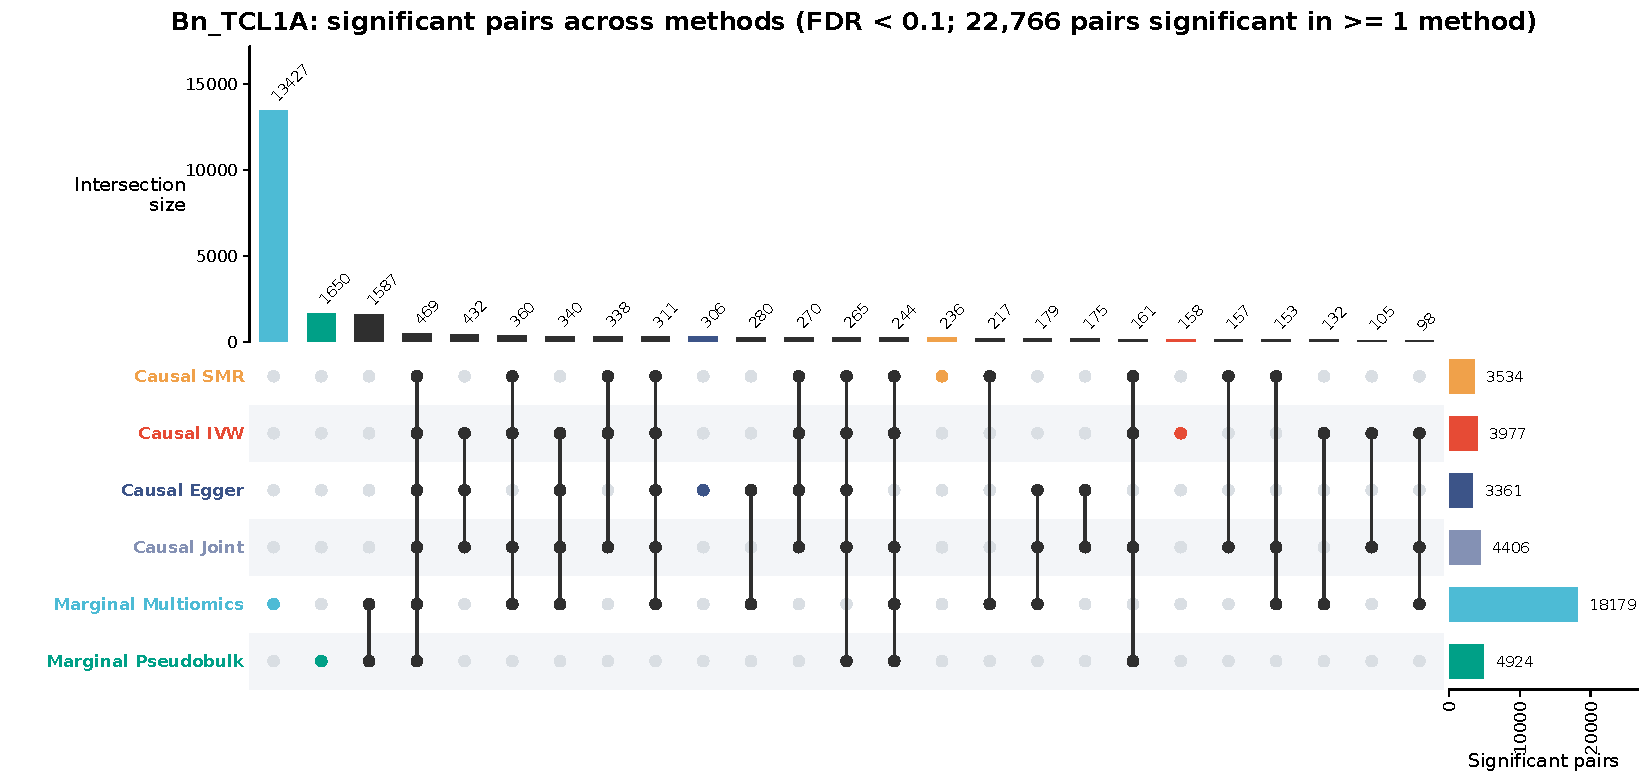
\includegraphics[page=1,width=\linewidth]{Fig1_MR_overview.pdf}\par\medskip
\includegraphics[page=4,width=\linewidth]{Fig1_MR_overview.pdf}
\caption{Overlap and direction of significant links. Top: Bn UpSet plot,
showing the 25 largest distinct significance combinations at \(\q<0.1\).
Bottom: effect-direction comparison among links significant in all six methods
in each cell type. Slices compare the IVW slope sign with the WNN and pseudobulk
correlation signs; central annotations summarize agreement among SMR, IVW,
and Egger. Existing source pages 1 and 4 are shown unchanged. The figure's
``Causal Joint'' label denotes CCT.}
\label{fig:overview}
\end{figure}

\begin{figure}[p]
\centering
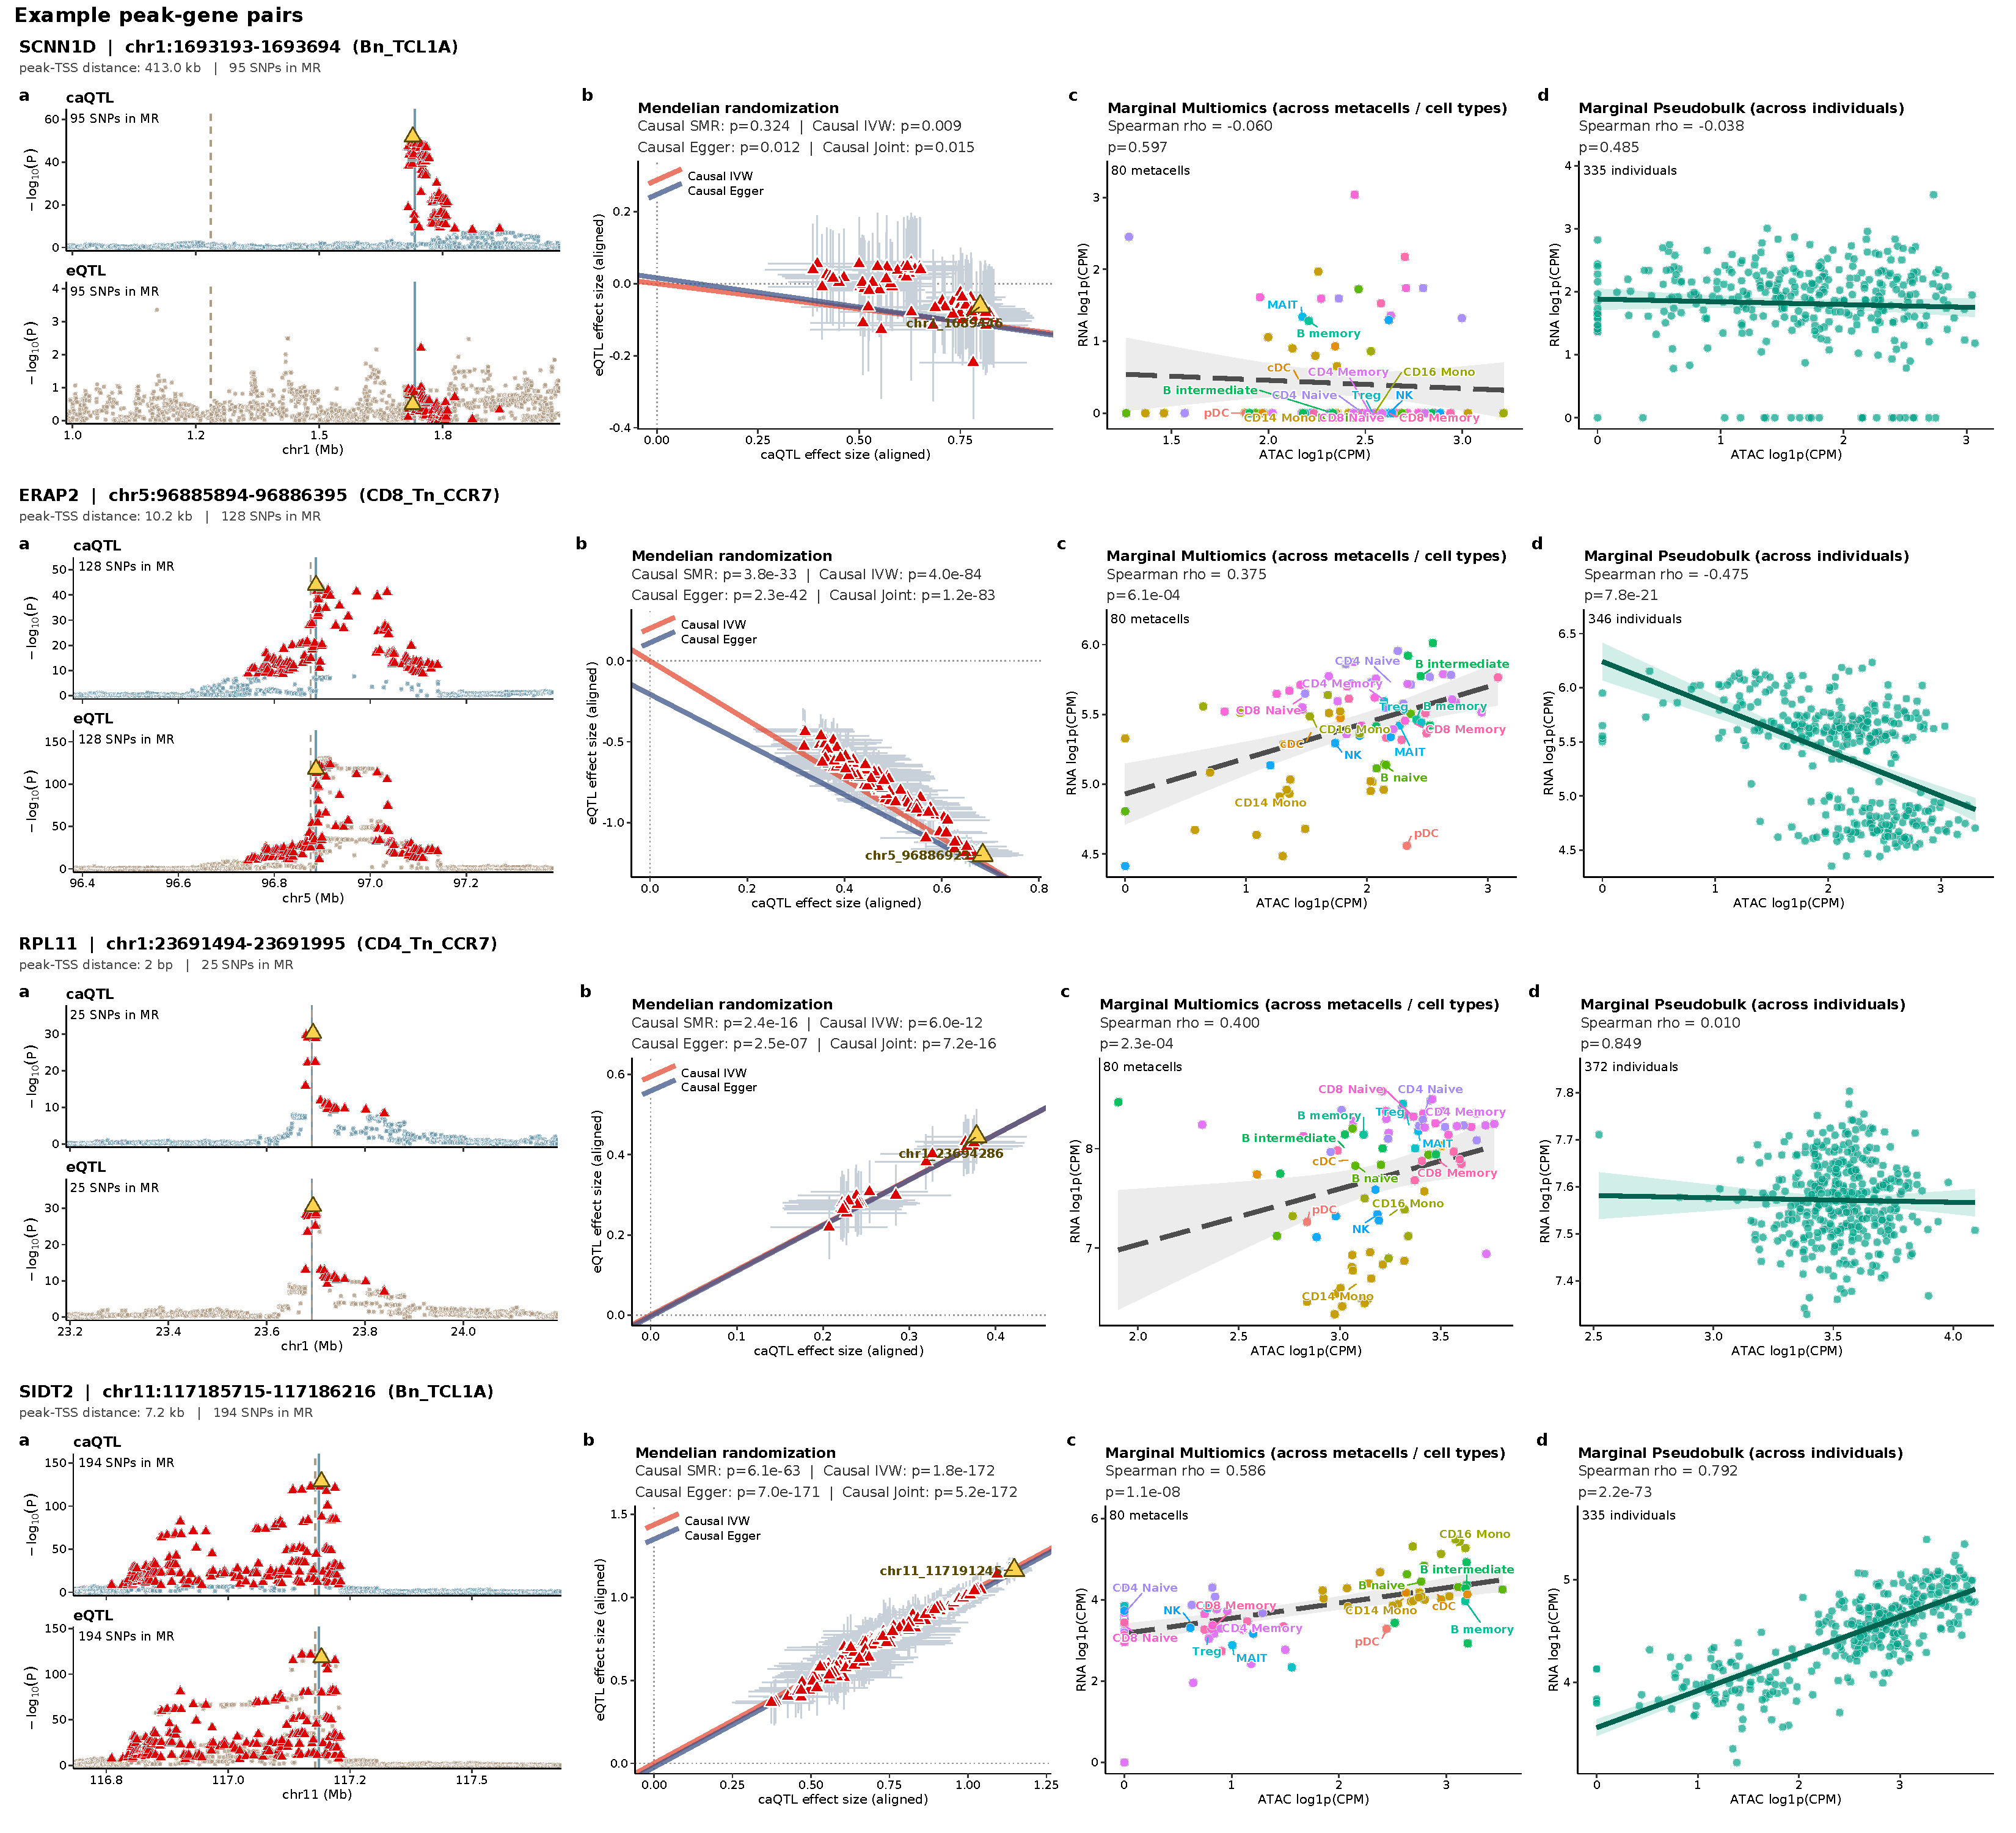
\includegraphics[page=1,width=\linewidth,height=0.79\textheight,keepaspectratio]{Fig2_examples.pdf}
\caption{Selected peak--gene examples: SCNN1D in Bn, ERAP2 in CD8, RPL11 in CD4,
and SIDT2 in Bn. Columns show QTL association tracks, aligned SNP effects with
IVW/Egger fitted lines, WNN metacell measurements, and pseudobulk measurements.
The displayed significance summaries are from the existing analysis; marginal
correlation summaries are Spearman correlations, while the drawn marginal
trend lines are linear fits. In the caQTL tracks, non-instrument variants with
\(p<10^{-8}\) are omitted by the original plotting script. Source page 1 is
shown unchanged; further examples remain in the copied six-page source PDF.
\textbf{TODO:} revise panel size and caption after example selection is reviewed.}
\label{fig:examples}
\end{figure}

\subsection{Regulatory reference support depends on the evaluation metric}
\label{res:references}
We evaluated links against EnhancerAtlas, FANTOM5, 4DGenome, GTEx, HiChIP, and
PCHiC reference datasets. The current pooled overlap summary reports enrichment
above one in every cell-type, method, and reference combination. SMR has the
largest pooled fold enrichment in 17 of 18 cell-type/reference combinations;
IVW has the largest value for CD4 PCHiC. In Bn, for example, SMR and WNN fold
enrichments are 6.18 and 3.56 against FANTOM5, and 4.46 and 3.08 against HiChIP.
The full existing summary is supplied as supporting Table~S1
(\texttt{Fig3\_Hyper\_table.xlsx}). These are descriptive comparisons of
method-specific selected sets, with different numbers of links and contributing
genes; they are not paired tests of method superiority.
% Evidence: Results/Figures/Figures_20261019/Fig3_Hyper_global.tsv.

We also summarized gene-wise ROC-AUC using raw-p-value significance scores
(Figure~\ref{fig:auc}). Differences in the stored mean AUCs were smaller and
benchmark-dependent. For Bn FANTOM5, mean AUC was 0.813 for SMR and 0.807 for
WNN, whereas for CD4 FANTOM5 it was 0.778 and 0.779, respectively. The existing
ROC calculations use automatic direction selection, so these summaries should
be read as the implemented benchmark rather than a fixed-direction ranking
comparison.
% Evidence: Results/Validation/Valid4_AUC/<CT>_AUC_long.tsv.gz.
\TODO{Select a compact reference-support table for the manuscript and develop
the interpretation of enrichment versus gene-wise discrimination.}

\begin{figure}[p]
\centering
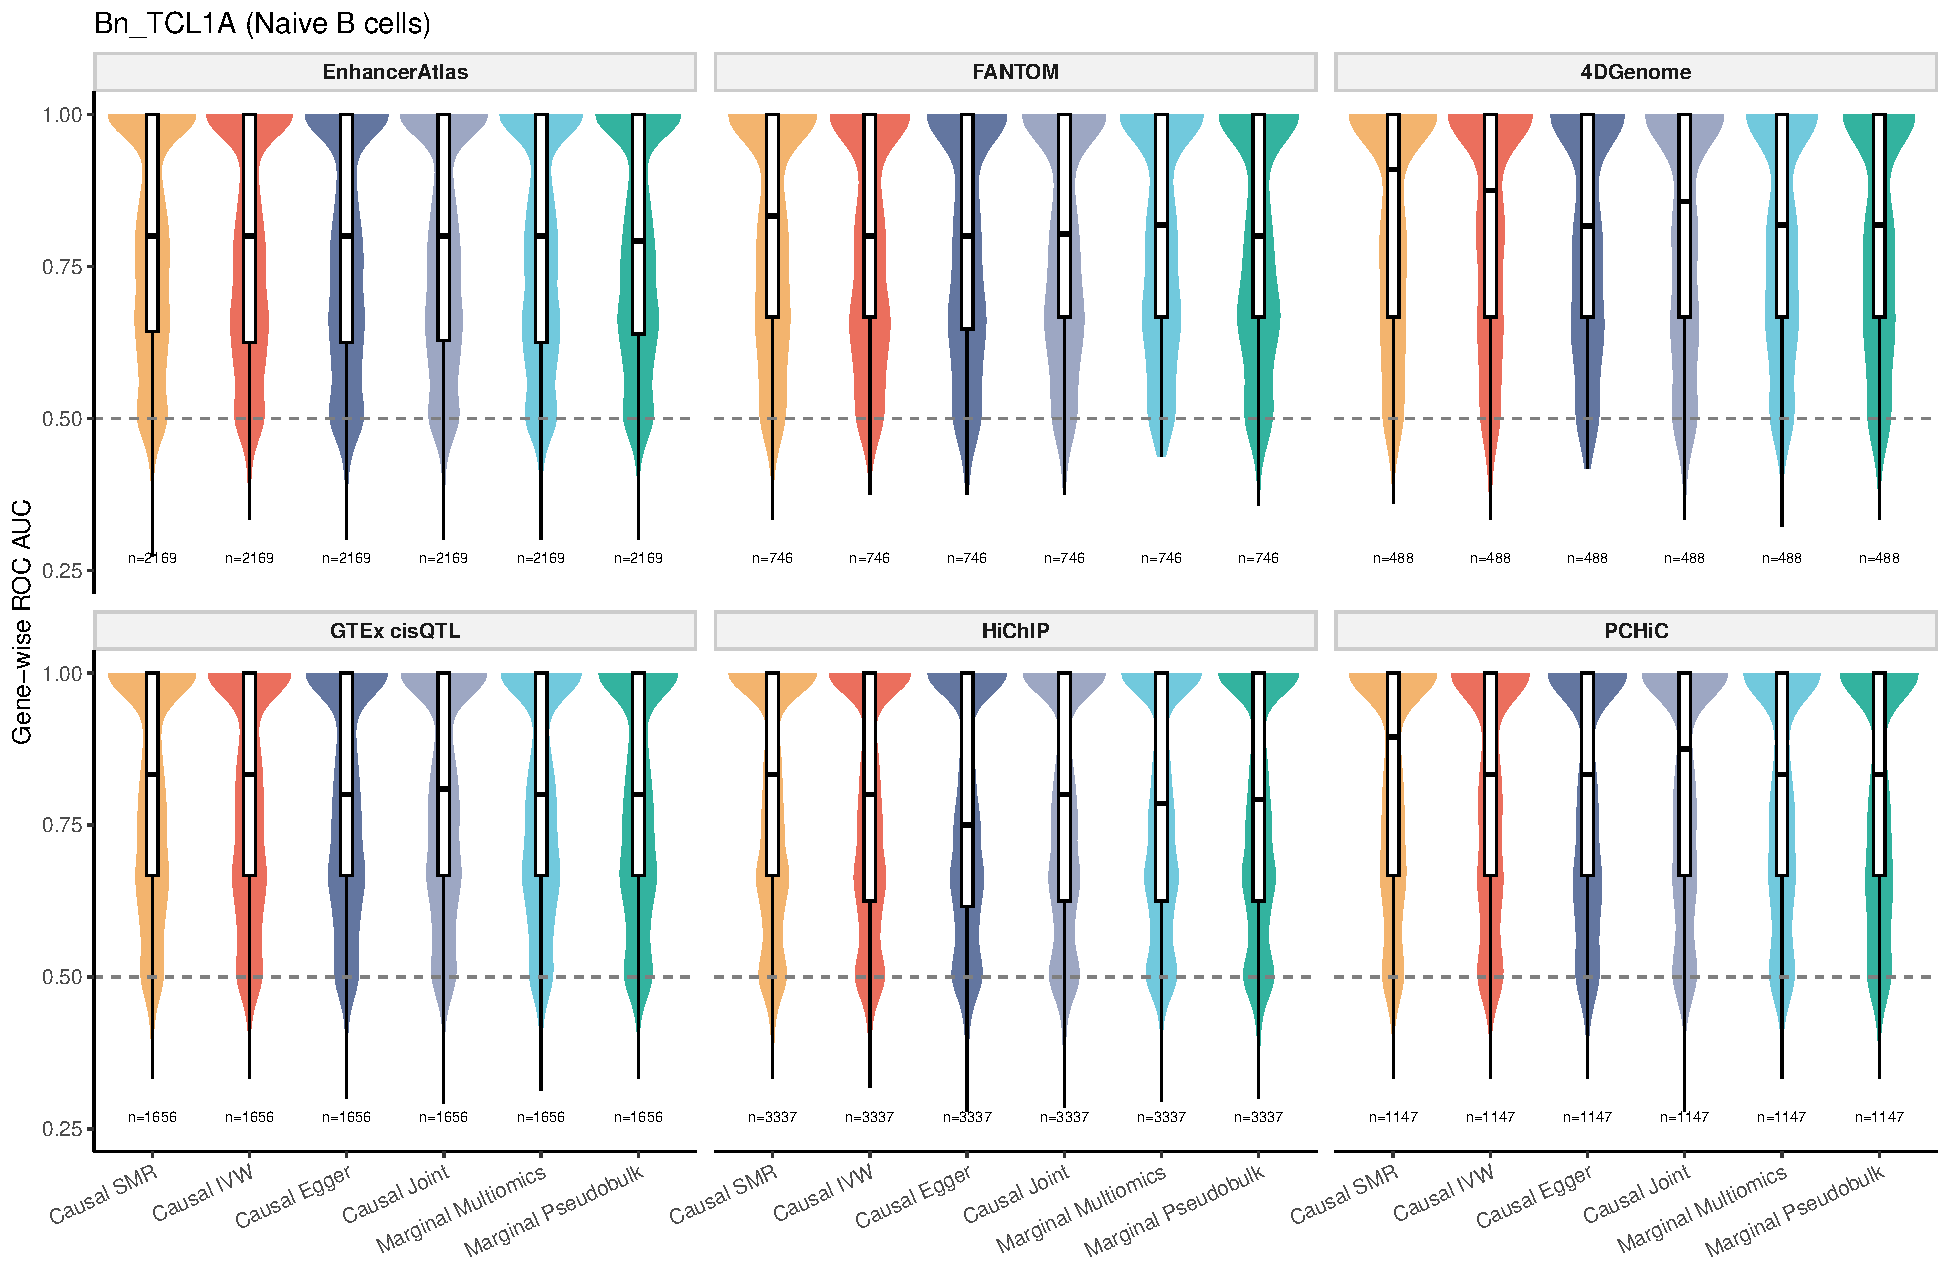
\includegraphics[page=1,width=\linewidth]{Fig4_AUC.pdf}
\caption{Gene-wise ROC-AUC against six regulatory references in Bn. Violin
and box plots summarize genes having both reference-overlapping and other
tested peaks; annotations give gene counts. Scores are \(-\log_{10}(p)\), and
ROC direction was selected automatically in the existing analysis. The dashed
line marks AUC 0.5. This is page 1 of the latest available AUC PDF, stored in
the older figure directory; CD4 and CD8 are retained as pages 2 and 3 of the
copied file.}
\label{fig:auc}
\end{figure}

\subsection{CIMA regulatory networks provide within-cohort corroboration}
\label{res:grn}
The cell-type-active CIMA SCENIC+ networks contained 864, 2,520, and 1,364
pairs from the retained Bn, CD4, and CD8 analysis sets, respectively.
At \(\q<0.05\), WNN had more network-overlapping significant pairs than SMR
(513 versus 324 in Bn), but SMR had a larger enrichment odds ratio
(9.60 versus 2.30 in Bn). This illustrates the distinction between overlap
counts and enrichment relative to the tested background
(Supplementary Figure~\ref{fig:supp-grn}). CIMA networks provide corroboration
within the same study, rather than independent experimental confirmation.
% Evidence: Valid5_GRN/GRN_summary.tsv and GRN_sig_counts_by_method.tsv.
\TODO{Integrate the high-quality eRegulon subset after deciding how much GRN
detail belongs in the main text.}

\subsection{Motifs and gene sets characterize functional relevance}
\label{res:function}
We examined motif enrichment in each method's significant peaks using
GC- and accessibility-matched backgrounds. Across 746 JASPAR motifs, the IVW
foreground yielded 58, 96, and 76 enriched motifs in Bn, CD4, and CD8,
respectively (BH-adjusted \(p<0.05\) and fold enrichment \(>1\)). The corresponding
WNN counts were 92, 123, and 92. These method-specific foregrounds are not
restricted to links unique to MR. TF-expression summaries and the existing
motif spreadsheet are supplied as supporting material (Table~S2).
% Evidence: Valid3_Motif/<CT>_motif_enrichment.tsv.gz; significance uses p.adjust.
\TODO{Choose representative TF motifs, verify their expression summaries, and
develop the biological interpretation; motif counts alone do not establish
functional specificity.}

For gene-set interpretation, we defined MR-only links as significant in at
least one of IVW, Egger, or SMR at \(\q<0.1\), with both marginal methods having
\(\q\geq0.1\). Their target genes numbered 1,581, 2,834, and 1,903, with 4,509
unique genes in the combined set. The existing GO Biological Process GSEA
returned no terms at conventional BH-adjusted \(p<0.1\) for individual cell
types, and nine for the combined set. Top combined terms include Arp2/3
complex-mediated actin nucleation and purine metabolism
(Supplementary Figure~\ref{fig:supp-go}). A separate 5,000-draw gene-set
resampling analysis returned 34, 213, 224, and 499 terms at empirical
BH-adjusted \(p<0.1\), respectively. These analyses use different null
comparisons and are kept distinct in this draft.
% Evidence: Valid7_GO/GO_GSEA_MROnly.tsv.gz; conventional p.adjust vs emp_fdr.
\TODO{Decide which GO comparison addresses the intended biological question
and select a small set of interpretable terms.}

\subsection{MR-only regions show exploratory disease-heritability enrichment}
\label{res:sldsc}
We used S-LDSC to examine peaks from MR-only links, with the definition above,
against nine immune-related GWAS. After liftOver to hg19, the MROnly sets
contained 1,271 Bn, 2,433 CD4, and 1,498 CD8 peaks; their union contained 3,777
peaks. Each extended peak annotation and the all-candidate-peak annotation
were fitted separately with baseline-LD annotations.

For the combined MROnly annotation, raw enrichment p-values were below 0.1
for Crohn's disease (CD), inflammatory bowel disease (IBD), multiple sclerosis
(MS), and type 1 diabetes (T1D), with enrichment estimates of 20.05, 18.04,
50.83, and 19.72, respectively (Figure~\ref{fig:sldsc}). Their raw p-values
ranged from 0.050 to 0.084; none met raw \(p<0.05\). These are exploratory
annotation-enrichment findings, without correction across the displayed
GWAS comparisons and without a direct test of MROnly versus all peaks.
% Evidence: Valid2_SLDSC/set_stats.tsv and SLDSC_all.tsv.
\TODO{Develop the disease interpretation and decide how to report uncertainty
alongside the existing figure, which omits standard-error bars.}

\begin{figure}[p]
\centering
\includegraphics[page=2,width=\linewidth]{Fig5_SLDSC.pdf}
\caption{S-LDSC enrichment for the union of the three cell-type MROnly peak
sets and the union of all candidate peaks. MROnly uses IVW/Egger/SMR link
\(\q<0.1\) and both marginal \(\q\geq0.1\). Peaks were lifted to hg19 and
extended by 500 bp on each side. Each custom annotation was fitted separately
with 97 baseline-LD annotations. Asterisks denote raw enrichment \(p<0.1\),
not multiplicity-adjusted significance or a test between the two bars.
AS: ankylosing spondylitis; CD: Crohn's disease; IBD: inflammatory bowel disease;
RA: rheumatoid arthritis; SLE: systemic lupus erythematosus; MS: multiple
sclerosis; T1D: type 1 diabetes; PBC: primary biliary cirrhosis, using the
source GWAS label. Source page 2 is unchanged; cell-type results are shown in
Supplementary Figure~\ref{fig:supp-sldsc}.}
\label{fig:sldsc}
\end{figure}

\subsection{GWAS-overlapping peaks nominate disease-associated regulatory examples}
\label{res:gwas}
For locus exploration, a separate, more stringent definition selected links
with any IVW, Egger, SMR, or CCT \(\q<0.001\) and both marginal \(\q\geq0.05\).
Requiring a GWAS variant with \(p<5\times10^{-8}\) inside the unextended peak
identified 27 cell-type-specific peak--gene pairs (7 Bn, 10 CD4, and 10 CD8),
covering 21 genes and 14 distinct peaks. The 37 output rows include repeated
pairs associated with different variant/trait records.

One example links the hg38 peak chr11:61827740--61828241 to TMEM258 in CD4
cells (Figure~\ref{fig:gwas}). SMR and IVW adjusted p-values were
\(2.39\times10^{-7}\) and \(8.21\times10^{-6}\), while WNN and pseudobulk
adjusted p-values were 0.398 and 0.225. The peak contains rs968567, associated
with asthma at \(p=3.67\times10^{-10}\). This positional overlap nominates a
candidate for follow-up; it does not establish colocalization or a mechanism
mediating disease risk.
% Evidence: Valid6_GWAS/GWAS_MRonly_overlap.tsv; source figure page 7.
\TODO{Review TMEM258 and alternative loci using appropriate biological
references before selecting the final disease example.}

\begin{figure}[p]
\centering
\includegraphics[page=7,width=\linewidth]{Fig8_Link_GWAS.pdf}
\caption{An asthma-associated peak linked to TMEM258 in CD4 cells. Tracks
show the gene, retained MR instruments, peak, and five method-specific links;
CCT is omitted in the original display. Solid links indicate \(\q<0.05\),
and dashed links indicate nonsignificance at that display threshold. The
purple symbol marks the overlapping GWAS variant rs968567. The x-axis is
rescaled around the peak and gene. This is unchanged source page 7 of the
27-page locus PDF; example selection remains provisional.}
\label{fig:gwas}
\end{figure}
